\documentclass[oneside]{nccuthesis}

\usepackage{times}
\usepackage{verbatim}
\usepackage{color}
\usepackage{url}
\usepackage{graphicx}
\usepackage{array}
\usepackage{pdfpages} % include outside .pdf
\usepackage{wallpaper} % watermark
\usepackage{tocloft}
\usepackage{xfrac}
% for table generate
\usepackage{mathtools}
\usepackage{amsmath}
\usepackage{amssymb}
\usepackage{booktabs}
\usepackage{diagbox}
\usepackage{adjustbox}
\usepackage{bm}
\usepackage{tcolorbox}

\usepackage{algorithm}
\usepackage{algpseudocode}
\usepackage{epsfig}

% Format the refs
\usepackage[sort,comma]{natbib}
\usepackage[hidelinks]{hyperref}
% For the tree
\usepackage{tikz}
\usepackage{tikz-qtree}

% For barchart
\usepackage{pgfplots}

% Using the tex-text mapping for ligatures etc.
\defaultfontfeatures{Mapping=tex-text}

% Set the default fonts
\setmainfont{Times New Roman}
\setCJKmainfont{標楷體-繁}

% Your information goes here
% Syntax: \var{English}{Chinese}
\university{}{國立政治大學}
\college{}{}
\institute{}{統計學系}
\title{Predicting Stock Returns via Greedy Algorithm with Taiwanese News Data}{在臺灣新聞資料下透過貪婪演算法預測股票報酬}
\author{Chang-Lei Cheng}{程長磊 \ 撰}
\studentid{110354030}
\advisor{Shi-Kui Lin, Ph.D.}{林士貴 \ 博士 \\[0.5ex] ~~~~~~~~~~~~~~~~~~~~翁久幸\ 博士}
\defenseyear{2023}{一一二}
\defensemonth{July}{7}
% \defenseday{15}

\pgfplotsset{compat=1.14}

\renewcommand\figurename{圖}
\renewcommand\tablename{表}
\renewcommand\contentsname{目錄}
\renewcommand\listfigurename{圖目錄}
\renewcommand\listtablename{表目錄}

% value > 0
\def\xeCJKembold{1}

% hack into xeCJK, you don't need to understand it
\def\saveCJKnode{\dimen255\lastkern}
\def\restoreCJKnode{\kern-\dimen255\kern\dimen255}

% save old definition of \CJKsymbol and \CJKpunctsymbol for CJK output
\let\CJKoldsymbol\CJKsymbol
\let\CJKoldpunctsymbol\CJKpunctsymbol

% Very Naive Chinese Number
  \DeclareRobustCommand{\naiveZhNum}[1]{
  \ifnum #1 = 1
  一
  \else \ifnum #1 = 2
  二
  \else \ifnum #1 = 3
  三
  \else \ifnum #1 = 4
  四
  \else \ifnum #1 = 5
  五
  \else \ifnum #1 = 6
  六
  \else \ifnum #1 = 7
  七
  \else \ifnum #1 = 8
  八
  \else \ifnum #1 = 9
  九
  \else
  #1
  \fi\fi\fi\fi\fi\fi\fi\fi\fi
  }

\titleformat{\chapter}{\centering\Huge\bfseries}{第\naiveZhNum{\thechapter}\,章}{1em}{}

\titleclass{\subsubsubsection}{straight}[\subsection]

\newcounter{subsubsubsection}[subsubsection]
\renewcommand\thesubsubsubsection{\thesubsubsection.\arabic{subsubsubsection}}
\renewcommand\theparagraph{\thesubsubsubsection.\arabic{paragraph}} % optional; useful if paragraphs are to be numbered

\titleformat{\subsubsubsection}
  {\normalfont\normalsize\bfseries}{\thesubsubsubsection}{1em}{}
\titlespacing*{\subsubsubsection}
{0pt}{3.25ex plus 1ex minus .2ex}{1.5ex plus .2ex}

\makeatletter
\renewcommand\paragraph{\@startsection{paragraph}{5}{\z@}%
  {3.25ex \@plus1ex \@minus.2ex}%
  {-1em}%
  {\normalfont\normalsize\bfseries}}
\renewcommand\subparagraph{\@startsection{subparagraph}{6}{\parindent}%
  {3.25ex \@plus1ex \@minus .2ex}%
  {-1em}%
  {\normalfont\normalsize\bfseries}}
\def\toclevel@subsubsubsection{4}
\def\toclevel@paragraph{5}
\def\toclevel@paragraph{6}
\def\l@subsubsubsection{\@dottedtocline{4}{7em}{4em}}
\def\l@paragraph{\@dottedtocline{5}{10em}{5em}}
\def\l@subparagraph{\@dottedtocline{6}{14em}{6em}}
\makeatother

\setcounter{secnumdepth}{4}
\setcounter{tocdepth}{4}

\begin{document}

% 政大論文浮水印
% % 政大論文浮水印
% \CenterWallPaper{0.174}{pdfs/watermark.pdf}
% \setlength{\wpXoffset}{6.1725cm}
% \setlength{\wpYoffset}{10.5225cm}

\CenterWallPaper{}{pdfs/watermark.pdf}
\setlength{\wpXoffset}{0pt}
\setlength{\wpYoffset}{0pt}

\hypersetup{pageanchor=false}

\frontmatter

\pagenumbering{gobble}

\makecover

\clearpages
\setcounter{page}{1}
\hypersetup{pageanchor=true}
\pagenumbering{roman}
\phantomsection

% generate certification
% \makecertification
% or include scanned pdf
% \addcontentsline{toc}{chapter}{口試委員會審定書}
% 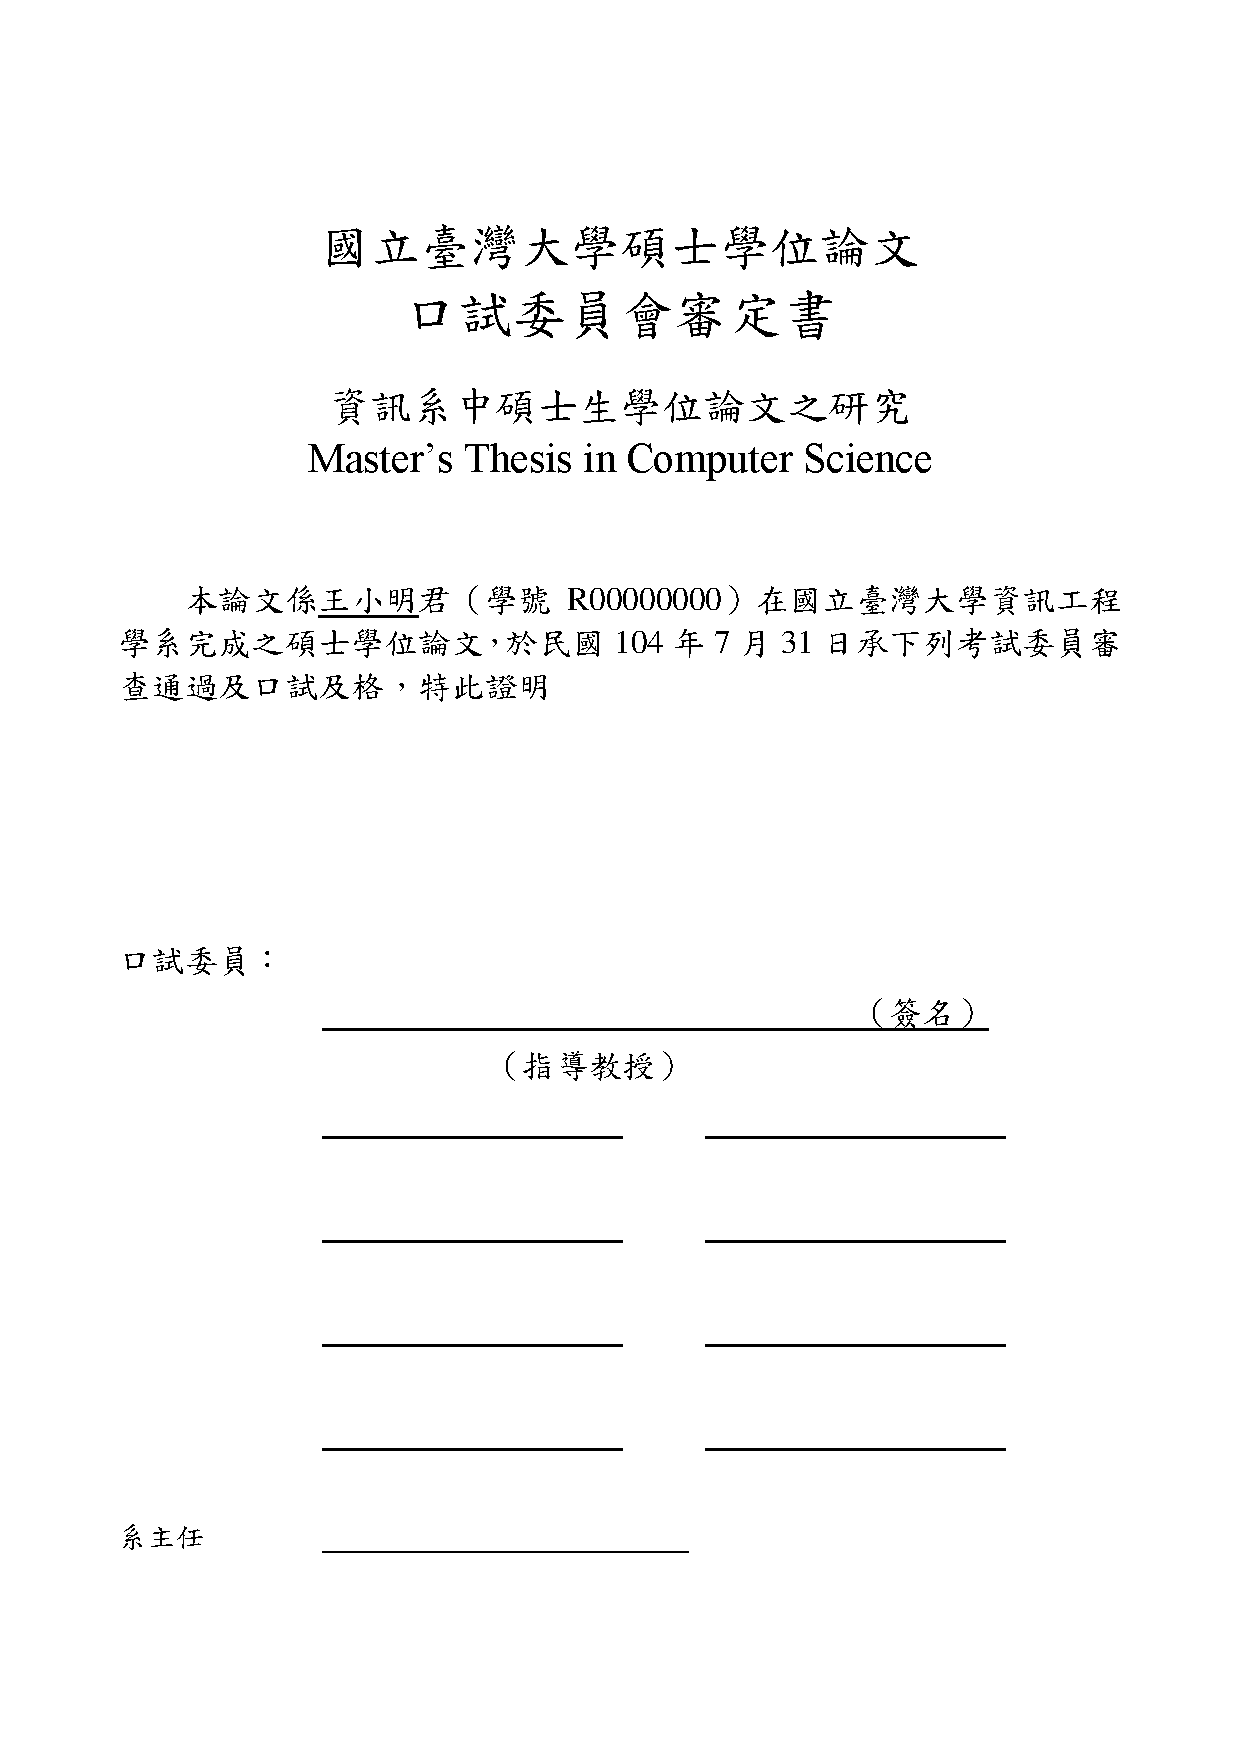
\includepdf[pages={1}]{pdfs/cert.pdf}

% \begin{acknowledgementszh}

\begin{flushright}
% 程長磊 \\
% 民國 一一二 年 六 月
\end{flushright}

\end{acknowledgementszh}

% \begin{acknowledgementsen}
 
% \end{acknowledgementsen}

 \begin{abstractzh}
隨著大數據、自然語言處理等領域發展,使得非結構化資料(Unstructured Data)具有極大的學術研究價值,尤其是文本資料。許多研究著手文字訊息對資產報酬之影響,使其成為財務領域中重要的研究目標之一,然而文本資料屬於高維度資料,如何正確分析文本資料與報酬間的關係成為此類研究的重要議題。而新聞文章是投資人在交易時最普遍接觸的文本資料,新聞文章與財報資料不同的地方在於新聞文章並沒有實際量化資料做為投資的依據,因此本研究欲透過Ing and Lai (2011)提出之 Orthogonal Greedy Algorithm (OGA) 以及由Chen, Dai, Ing, Lai (2019) 所改良之Chebyshev Greedy Algorithm (CGA) 高維度選模模型,挑選新聞中常用字詞之文字探勘方法以量化新聞文章之情緒分數,並在排除公司報酬因子下計算新聞情緒因子與公司報酬間之關係,並比較當應變數報酬為線性或是非線性的假設之下,利用新聞情緒分數所建構之投資組合之報酬差異。在應變數報酬為連續變數之線性假設下使用 OGA 並推廣為 OGA Predict模型,而在應變數報酬為非線性假設下則使用CGA並推廣為CGA Predict模型,並將上述兩種選模方法創新應用於財務文本分析之中。我們發現相較於OGA Predict,CGA predict模型可以得到更好的超額報酬,同時透過績效評估發現,新聞文章情緒對於散戶投資人為主的臺灣市場之影響與法人投資人為主的美國市場相比是顯著不同的,其結果也符合我們對於臺灣股票市場的經濟直觀。
~\\
\par
\noindent 
關鍵字:
\par
\noindent 文字探勘、統計學習、新聞情緒分析、預測股票報酬、OGA、CGA
\end{abstractzh}



\begin{abstracten}
The development of unstructured data grows fast and has the value of research along with the improvement of the realm of big data, especially for textual data. However, textual data are high dimensional data (i.e. the number of text in the news articles far exceeded than the news articles themselves.), therefore analyzing the relationship between textual data and the average return correctly has been an important issue according to this realm of research. When trading, the textual data that are most commonly received by investors are news articles. The difference between news articles and financial statements is that news articles can not provide quantitative information as an investment foundation. Therefore, we suppose to use two different kinds of high dimensional model selection methods, Orthogonal Greedy Algorithm(Ing and Lai (2011)) and Chebyshev Greedy Algorithm(Chen, Dai, Ing, Lai(2019)), and then select the frequently use words from news articles in order to quantify the sentiment scores of news articles. Moreover, we compare the difference of the portfolio returns which are constructed under two different assumptions(linear or nonlinear) of dependent variables according to the news sentiments. We use the OGA predict model to construct news sentiment when the dependent variable is under linear assumption, otherwise, we use the CGA predict. We find that the average return from the CGA predict model is better than the average return from the OGA predict model. Moreover, there is a significant difference in decision making when trading between the Taiwanese market and US market.


\par
\noindent
\textbf{Keywords:}
\par
\noindent
Text mining、Statistical Learning、News Sentiment Analysis、Stock Returns Prediction、OGA、CGA
\end{abstracten}


% Table of Content
\clearpages
\tableofcontents
% List of Figures
\clearpages
\listoffigures
% List of Tables
\clearpages
\listoftables

\mainmatter


% Your thesis goes here
\chapter{緒論}
\label{c:intro}

\section{研究背景}
根據國際數據資訊公司(IDC)表示,在2024年前每年所產生、捕捉、複製、消耗的資料總量將會超過 149 ZB,且多數是非結構化資料,若能具備分析非結構化資料的能力,將能為公司帶來極高的價值。Seagate 預估,到了2025年我們所接觸到的資料中有八成將會是非結構化資料,非結構化資料不僅數量龐大且具有極大的學術發展及商業價值。

根據 IBM 定義,結構化數據(Structured Data)為高度組織化並且易透過機器學習等演算法進行處理的一種資料型態。其優點為不需深入了解不同類型之數據及運作方式,即可做進一步的處理與解釋。然而其缺點為受限之靈活與可用性,結構化資料需儲存於固定格式之數據儲存系統中(如: SQL),若數據需求有所變化時,則必須更新所有數據進而導致大量時間與資源的消耗。而非結構化數據 (Unstructured Data) (包括文字、聲音、圖片、影像等)則無法透過傳統的數據分析方法進行分析。非結構化資料之優勢為可保持未
定義之原始型態,具較高適應性且不需預先定義數據,因此可以更快速且更輕鬆的收集數據而擴大數據池,使資料科學家進行更全面與深入的分析。然而其缺點則為,由於其未定義與非格式化之性質,處理非結構化數據時需仰賴專業知識,如何有效處理非結構化數據成為研究中重要的領域。

而文字訊息對資產報酬的影響早已是財務領域中重要的研究議題。過往研究學者發現市場價格與交易量會受投資者解讀訊息之差異而受影響,認為市場是由理性投資者及非理性投資者組成,而非理性投資者於市場上蒐集訊息,以符合自身對於該資產之預期信念,不同投資者對於訊息的解讀想法將導致不同的決策行為,進而影響相對應的資產價格與市場活動。隨著訊息傳遞研究之發展,實證分析中發現影響投資者決策之訊息中以媒體內容最具影響性,解讀媒體內容後之情緒反應可視為影響資產價格之重要變數,媒體內容、公司之知名度可增加投資者投資該公司的想法 (Merton (1987)、De Long, Shleifer, Summers, and Waldmann (1990a)、Mullainathan and Shleifer (2005)、Duffie (2010))。另從投資者接受媒體內容之特性與理解度進行分析,結果顯示投資者常常只關注廣泛一般訊息,而忽略需要花時間人為處理的詳細訊息,也較易混淆媒體之陳舊程度。因此取得先行消息之投資者可利用消息不對稱的優勢先行決策,使得投資者對於內容之反應具有偏差,因此市場常發生反應落後或過度反應等不效率現象。

整理過去之模型設計,總共可以分成三個類型:分別為建構字典、機器學習法與計量統計模型。建構字典之方法始於傳統語言學,以人工方式編輯成字典;機器學習法與統計計量模型則以 “Learning From Data” 為目標,透過資料處理與模型設計,對資料做進一步的分析。

現今,自然語言處理在許多不同的領域已有很大的發展,然而文本分析應用於財務領域之實證分析仍有很大的進步空間。在財務文字探勘領域,研究文本資料之「情緒」並利用各種不同的方法將其量化為情緒分數(Sentiment Score)為主要研究方向,情感分數可以透過特定方法量化數據後估算而得(e.g. Harvard-IV 社會心理學詞典),接著建構統計模型,並可用於研究財務消息面於金融市場之傳遞情形與不同消息接收度所帶來之影響。

\newpage

\section{研究動機與目的}
最初財務文本使用建構情緒字典方式量化文字情緒,而其缺點為需高度的仰賴人工主觀選字,難以消化隨著時代不斷增加之非結構化資料,也無法因應不斷產生之新詞彙,在預測時無法時時刻刻精確。

有學者提出使用機器學習方法量化文字情緒,然而機器學習模型設計複雜且解釋性不及建構字典法與統計計量方法,因此亦有學著嘗試建構統計計量模型以設計文字情緒量化模型。

近幾年高維度資料問題興起,當解釋變數數量超過所觀測到之樣本數時,標準的迴歸模型(OLS)存在計算上與理論上估計之困難,Ing and Lai (2011) 改良最小平方逐步迴歸法提出 Orthogonal Greedy Algorithm (OGA)解決此類問題,然而該研究尚未應用於具低訊雜比(Signal-to-Noise Ratio)特性之財務文字資料研究上,而與舊有之統計模型相比較(如:SESTM、FARM Predict),執行OGA時電腦所需之運算時間大幅下降,也有足夠的解釋性。本研究預計使用OGA模型於文字情緒量化上之研究並創新應用於文本分析之 OGA Predict 模型;上述之選模方法是建立在當應變數為線性假設之連續報酬的情況下,然而許多文獻支持以二分類報酬(令漲為1、跌或平盤為0)做為文字情緒量化研究之應變數(Fan, et al. (2020), Fan, et al. (2021), Jiang, et al. (2020)),因此本研究也預計使用 Chen, et al.(2019) 改良 CGA 之延伸方法 Chebyshev Greedy Algorithm (CGA) 針對二分類報酬進行建模,並推廣至 CGA Predict 財務文本模型,並基於兩種方法探討在應變數報酬為線性假設或非線性假設的情況下有何異同,並驗證台灣股票市場中之散戶於市場中之反應與績效表現。
\chapter{文獻回顧}
利用文字探勘方法分析金融市場早已是財務領域重要的研究方向。本章聚焦於財務文本分析之發展,從傳統的字典方法、機器學習至現今所使用的統計計量模型,並探討本研究所使用之統計學習方法 Orthogonal Greedy Algorithm (以下稱 OGA) 以及 Chebyshev Greedy Algorithm (以下稱 CGA)之發展。
\section{財務文本分析}
\subsection{傳統字典方法}
最早應用於財務領域之文字情緒量化模型以建構情緒辭典為主要方法,以 Tetlock (2007)所提出之Harvard-IV辭典為例。該研究從Harvard-IV辭典中選出77個具有相對頻率的負向辭彙並將其分為強、中、弱等類別,實證分析採用<<華爾街日報>>之新聞文章,結果顯示包含負面情緒之新聞文章對於報酬有顯著的影響,發現於發佈新聞當日,道瓊工業平均指數下降了8.1 bps,結果也證實負面消息與正面消息相比較,負面消息影響較大也較全面。

Loughran and McDonald (2011)發現在Tetlock (2007)所提出之辭典中有將近百分之七十五之字詞與財務上常使用之字詞相去甚遠。為了改善Harvard-IV辭典以簡單計數挑選出情緒字詞而量化新聞文章情緒的方式,使用了大量美國10K公司年度財報中的資料,建構出更貼近於金融市場所使用的字詞之辭典,其中包含報酬、交易量等基本財務資訊,使得量化後之情緒分數得以更貼近於真實的情緒。Jeon, McCurdy, and Zhao (2021) 結合 Loughran and McDonald (2011)之辭典並加入了橫截面迴歸與邏吉斯迴歸等方法,發現股票收益跳躍、新聞發佈頻率等二者與內容之相關性顯著,且對於具有較高媒體知名度、分析師覆蓋率和機構所有權的公司,跳躍機率對新聞具有更高的敏感性。

量化文字情緒最簡單快速的方式是為建構情緒辭典,大部分關鍵字詞在財務意義上皆具其合理性與解釋性。然則,建構情緒辭典需依賴大量的主觀選字,在實務上難以消化與解釋大量非結構化資料所產生的特定情緒字詞,也無法因應因時代快速變遷所產生之新詞彙。隨著電腦運算速度提升與機器學習之發展,許多學者研究以機器學習方法量化文本資料之量化模型。
\subsection{機器學習方法}
最早的文字探勘研究主要集中在文本分類和訊息搜索等領域,其中一個重要的成果是樸素貝氏分類器(Naive Bayes Classifier),Paul Graham (2002) 探討了傳統的垃圾郵件過濾方法的不足之處,並提出了一種基於貝氏定理的過濾方法,並且在實驗中取得了不錯的效果。此分類方法被廣泛應用於文本分類、情感分析等領域,並成為自然語言處理中一個重要的基礎技術。

Gentzkow, Kelly, and Taddy (2019) 透過 Bayesian Regression, Nonlinear Text Regression, Generative Language Models, Word Embeddings等模型進行比較,認為利用機器學習模型可以將文本中有用之訊息轉換為可進行因果分析之量化形式,並將其應用於股票市場的預測、衡量央行演講的情緒與分析媒體內容的政治傾向。

隨著Web的興起,文本資料量急劇增加,文字探勘進入快速發展期,此時出現了新的技術與模型,如主題模型(Topic Model)、情感分析(Sentiment Analysis)和文本摘要(Text Summarization)等。隨著機器學習算法的進步,文字探勘的研究開始轉向基於統計和機器學習的方法,其中一個重要的發展是Tomas Mikolov, Kai Chen, Greg Corrado, and Jeffrey Dean (2013) 首次提出的 Word2Vec 模型,該模型包括Skip-Gram和CBOW兩種訓練方式,通過大量的文本數據來學習單詞並將單詞轉換為向量表示且具有較高的計算效率,以達到更精確的文本分析。

至於台灣新聞資料的分析中,以 Tien (2019) 使用鉅亨網台灣股市新聞資料進行文本情緒分析為例,其利用了機器學習與深度學習等模型,主要研究文本資料的前處理以及搭配文本分類模型之分類效果的好壞,結果顯示深度學習模型在文字情緒分析上具有較高的準確度與模型穩定性;N-gram字詞特徵提取在三種分類模型中皆能提升準確率,特別是應用在Naive Bayes的分類器上,可以有效地改善需要對模型進行假設的缺點。

機器學習的優勢在於能夠在眾多參數組合的模型中進行搜索,並有效地選擇重要變數與降低模型維度,惟機器學習模型設計複雜較難以解釋且有黑盒子等問題存在,因此有研究使用統計計量模型建構文字量化模型。

\subsection{統計計量模型}
統計計量模型主要貢獻在於建構具有良好統計性質之文字模型,解決了在文字資料常存在之高維度與稀疏性的問題,相較於機器學習模型來說其設計的更簡單且更具有解釋性。

Ke, Kelly, and Xiu (2019)提出Sentiment Extraction via Screening and Topic Modeling (SESTM) 模型,以解決過去情緒辭典模型無法隨著時代演進而更新之動態更新問題;該模型簡單、運算快速且經證明具有良好的統計性質,解決了機器學習模型難以解釋的缺點。實證上使用Dow Jones Newswire研究美國股票市場,該資料集長度、內容完整且具代表性,解決了過去大多文獻只使用少部分資料集測試的問題。Fan, Xue, and Zhou(2021)改進Ke, Kelly, and Xiu (2019)之SESTM模型需對於文字情緒與股價報酬進行過於強烈的假設與監督式學習需要過度依賴過去資料之缺點,提出Factor-Augmented Regularized Model for Prediction (FARM Preict) 模型;其模型以非監督學習的方式從每篇文章中選取重要的字詞做為因子,並分析了中文字詞與英文字詞之間表義與拼音的差異。實證上應用於中國新聞資料庫:<<新浪>>財經新聞,實證結果發現中國市場以散戶投資人為主,相較於正面消息,散戶投資人對於負面的新聞消息具有更大的反應,然而由於政府在放空上有所限制,所以散戶投資人對於負面消息的反應無法反映在投資組合之報酬之中。透過個股新聞資料所計算之情緒分數不僅能確切反應個股報酬且將不受過去股價所影響。


\section{高維度選模方法}
由於非結構化資料的發展與演進,如何有效地處理高維度資料所帶來的問題逐漸浮現,所謂高維度資料,也就是當變數數量超過所觀測到的樣本數時,如果使用標準的迴歸模型估計迴歸係數時,在計算與估計上會有困難(例如:高維度反矩陣不存在)。過往文獻多為透過$L_1$懲罰項之最小平方法($L_1$-Penalized Least Squares)來解決此問題。Tibshirani(1996)首先提出Lasso Regression,並應用於迴歸選模的問題。Lasso主要的使用方法為在目標式中加入係數絕對值總和作為懲罰項(Penalty term),迫使不相關之係數為0,進而得到一個具有解釋能力的模型。Bü hlmann and Yu (2003)提出$L_2$-boosting,其為基於$L_2$損失函數之梯度下降法所建構之演算法,他們證實在高維度的問題之中,使用立方平滑曲線的$L_2$-boosting是有效且能實踐的。

%Efron, Hastie, Johnstone, and Tibshirani (2004)基於傳統向前選取法(Forward Selection)進行改良,提出更有效之選模方法:Least Angel Regression (LARS)。LARS連結了Lasso與Forward Selection Regression,主要有三大特點:第一,他可以很容易實踐出lasso方法並且花費更少的時間;第二,不同之LARS修改能有效地實踐出向前選取迴歸(Forward Selection Regression);第三,可以很容易的估計出LARS的自由度。
Stepwise Least Square Regression為一個被用以處理大量解釋變數之迴歸分析演算法,由以下三個特性所組成:一,以貪婪(Greedy)的方式進行向前選取,同時將挑選出來的變數與先前挑選的變數進行最小平方迴歸,目的在於最小化殘差平方和(Residual Sum of Squares);第二,擁有中斷向前選取之規則 (Stopping Rule);第三,擁有根據一些自訂之準則而向後(Backward selection)刪除所挑選出之變數,以最大化變數與應變數之間的相關性。Ing and Lai (2011)針對高維度迴歸問題,有別於過往使用$L_1$懲罰項之最小平方法,提出在稀疏條件下(Sparsity Condition)基於 Forward Stepwise Component 之高維度迴歸選模演算法 OGA。Ing and Lai (2011) 同時開發出快速迭代過程用以更新 OGA process,因此 OGA 選模與先前所提及之演算法相比擁有更快的運算速度。

本計畫預計將此方法創新並應用於財務文本資料的分析,因 OGA 可以針對超額報酬下挑選重要相關字詞進而建構投資組合。而當報酬為二分類報酬(例如:上漲時設為1,下跌或平盤時設為0),此時必須使用邏吉斯迴歸模型取代原本於 OGA 模型所使用之線性迴歸模型假設。Temlyakov (2015) 首先提出 CGA 近似方法解決凸形優化問題(Convex Optimization Problem),也就是說有別以往傳統線性選模問題提升至當損失函數滿足 Convex 特性時有遵循之選模方法。Chen, Dai, Ing, Lai (2019)
則將此CGA方法推廣至高維度下非線性選模演算法(High Dimensional CGA),因此本計畫透過CGA解決當應變數報酬為二分類報酬時之文本分析問題。

\chapter{研究方法}
OGA 模型之優點在於:第一,OGA 不需要過於嚴格的假 設條件,只要應變數為線性假設即可;第二,OGA 透過線性迴歸挑選與應變數相關性較高之解釋變數,因此 OGA 模型具有很好的解釋性以及快速的運算速度。而為了研究當應變數為非線性假設時之選模問題,本研究使用 CGA 模型取代 OGA 模型,CGA 保留了 OGA 的優點並將線性模型推廣至非線性模型,以解決應變數為二分類報酬下之邏吉斯迴歸選模問題。
\section{資料結構}
本研究中收集每篇均有明確標記所對應之個股名稱與代號之新聞文章並建構一個$n$篇新聞文章及$p$個字詞的字詞矩陣,將字詞出現於第$i^{th}$篇新聞文章的次數以字詞計數向量$x_i \in R_+^m$表示。其中 $x_{i,j}$ 則表示字詞$j$在第$i$篇文章中出現的次數$i = 1,2,··· ,n\text{,  }j = 1,2,··· ,p$,此字詞數量向量以矩陣形式(Document-term Matrix)表示如下:
\begin{equation}
X=\begin{pmatrix*}
x_{1,1} & \cdots & x_{1,p} \\
\vdots & \ddots & \vdots \\
x_{n,1} & \cdots & x_{n,p}
\end{pmatrix*}
\end{equation}
{其中$x_{i,j}$ 表示字詞 $j$ 在第 $i^{th}$  篇文章中出現的次數,$y_i$表示第$i^{th}$篇新聞所標記之股票報酬。本研究之研究目的為分析個股新聞情緒是否影響個股報酬,由於模型限制等因素,需移除未標記股票之新聞、標記多於一支股票之新聞、重複新聞與公告類新聞,以維持字詞數量矩陣與目標股票報酬具一對一之關係。由於在一篇文章中每個字詞出現的頻率不盡相同,為了減少出現頻率過少的字詞影響模型估計結果並簡化模型,根據 Fan, Xue, and Zhou (2021) 之建議,透過設定閾值 $\kappa$ ,設定字詞至少出現之次數以減少模型之雜訊(noise),其公式如下:
}
\begin{equation}
X^{freq}=\{j^{th}~\text{word in}~\bm{X}:k_j \geq \kappa \}
\end{equation}
\section{Pure Greedy Algorithm}
\subsection{迴歸模型設定}
\noindent
考慮線性迴歸模型:
\begin{equation}
\displaystyle y_{i}=\alpha + \sum^{p}_{j=1} \beta_{j}x_{ij}+\varepsilon_{i}, i=1,\ldots,n
\end{equation}
其中$x_{i1},x_{i2},\ldots,x_{ip}$為模型中之$p$個解釋變數,當$p > n$時(i.e. 解釋變數數量大於所觀測到之樣本數量),使用標準的線性迴歸模型估計迴歸係數時存在計算與統計估計上的困難,然而許多研究證實在稀疏性的條件(Sparsity Condition)成立之下,此時迴歸模型:
\begin{equation}
y(x)=\alpha+\beta^{\top}x, where~\beta=(\beta_{1},\beta_{2},\ldots,\beta_{p})^{\top}, x=(x_{1},x_{2},...,x_{p})^{\top}
\end{equation}
之一致性估計(Consistency Estimation) 仍然有可能存在。

\subsection{PGA process}
在介紹Orthogonal Greedy Algorithm (以下稱OGA)之前,我們需要對Pure Greedy Algorithm (以下稱PGA)選模步驟有初步的認識。PGA為一種逐步迴歸 (Forward Stepwise Regression) 法,由 Bühlmann and Yu (2003) 所提出,PGA選模步驟是透過迭代後生成之殘差,進行分量線性最小平方法而生成迴歸式線性近似值之過程。首先將$y_{i}$與$x_{ij}$分別以$y_{i}-\overline{y}$, $x_{i}-\overline{x}$取代,並假設$\alpha = 0$,使得:
\begin{equation}
\displaystyle y_{i} = \sum_{j=1}^{p} \beta_{j}x_{ij}+\varepsilon_i, i=1,2,\ldots,n 
\end{equation}
,初始化近似值$ \hat{y}_0(x)=0$ (when $k=0$),並在每次迭代結束後計算殘差:
\begin{equation}
U_i^{(k)}=y_i - \hat{y}_i(x_i),1\leq i \leq n
\end{equation}
,計算完殘差之後挑選 $ x_{i,\hat{j}_{k+1}} $ 與殘差跑迴歸,使得:
\begin{equation}
\displaystyle \hat{j}_{k+1}=argmin_{1\leq j \leq p}\sum_{i=1}^{n}(U_i^{(k)}-\tilde{\beta}_j^{(k)}x_{ij})^2,
\end{equation}
where $\displaystyle \tilde{\beta}_j^{(k)}=\sum_{i=1}^{n} U_i^{(k)x_{ij}} / \sum_{i=1}^{n}x_{ij}^2 $。最後更新近似值:
\begin{equation}
\hat{y}_{k+1}(x)=\hat{y}_{k}(x)+ \tilde{\beta}_j^{(k)}x_{\hat{J}_{k+1}}
\end{equation}
重複上述迭代步驟直到達到預先指定的迭代上限$m$。特別注意,PGA 在每次的迭代過程中,由於沒有針對模型做特定的假設,使得PGA模型是有可能挑選到重複變數的。

\newpage

\section{Orthogonal Greedy Algorithm}
\subsection{OGA process}
Orthogonal Greedy Algorithm (OGA) 模型由 Ing and Lai (2011) 提出,是一種高維度稀疏迴歸模型 (High-dimensional Sparse Regression)之選模方法。

OGA之迴歸模型設定與PGA之迴歸模型設定(式3.3)相同,由於
\begin{equation}
\displaystyle \frac{\sum^{n}_{i=1}(U_i^{(k)}-\tilde{\beta}_j^{(k)}x_{ij})^2}{\sum_{i=1}^{n}(U_i^{(k)})^2}=1-r_j^2
\end{equation}
,其中$r_{j}$為$x_{ij}$與$U_i^{(k)}$之相關係數,因此前述之選模方法等價於在各個迭代過程中挑選與$U_i^{(k)}$相關性最高之解釋變數。而 OGA 的實現是以另一種方式更新近似值,並對向量$ X_{\hat{j}_{k+1}} $進行正交轉換至$ X_{\hat{j}_{k+1}}^{\bot} $,並使用以下更新方式:
\begin{equation}
\hat{y}_{k+1}(x)=\hat{y}_{k}(x)+ \tilde{\beta}_j^{(k)}x_{\hat{J}_{k+1}}^{\bot}, 
\end{equation}
where $\displaystyle \tilde{\beta}_j^{(k)}=\sum_{i=1}^{n} U_i^{(k)}x_{i,\hat{J}_{k+1}}^\bot / \sum_{i=1}^{n}(x_{i,\hat{J}_{k+1}}^\bot)^2$
,藉由依序將解釋變數正交化,如此一來通過分量線性迴歸(Componentwise Linear Regression)來使用最小平方法估計參數,進而避免高維度的反矩陣不存在導致有估計上困難的問題。(Ing and Lai (2011))

由於OGA中挑選$U_i^{(k)}$相關性最強的解釋變數等價於$y_{i}$對$(x_{i,\hat{J}_1},\ldots,x_{i,\hat{J}_k+1})$,然而$U_i^{(k)}$是OGA中$y_{i}$對$(x_{i,\hat{J}_1},\ldots,x_{i,\hat{J}_k+1})$做最小平方迴歸的殘差,代表在選模過程中所選出之$\hat{J}_{k+1}$不會重複被選到(i.e. $j \notin \{\hat{J}_{1},\ldots,\hat{J}_{k+1}\}$)。所以 OGA 與 PGA 選模過程中不同的地方在於,PGA 有可能選到重複的變數而 OGA 則是排除了已經包括在{$\hat{J}_{k+1}$}中所考慮之變數。


\subsection{High Dimensional Information Criterion (HDIC)}
OGA迭代後,迴歸模型中總共有 k 個輸入變數,接下來沿著OGA路徑選擇一個具有最小高維度訊息量準則(HDIC)之模型。令$\hat{\sigma}^{2}_{J} = \frac{1}{n}\sum_{i=1}^{n}(y_i - \hat{y}_{i;J})^{2}$,其中$\hat{y}_{i;J}$代表當$Y$投影到由$X_{J}$所生成的線性空間中$y_{i}$的配適值,定義:
\begin{equation}
HDIC(J) = nlog(\hat{\sigma}^{2}_{J})+\#(J)w_nlog(p)
\end{equation}
\begin{equation}
k_n = argmin_{1\leq k \leq K_n}HDIC(\hat{J}_k)
\end{equation}
其中$\#(\cdot)$代表集合的數量,$\hat{J}_{k}=\{\hat{J}_1,\ldots,\hat{J}_k\}$。而根據不同的對應準則會有不同的$w_{n}$:$HDBIC:w_{n}=logn$適合強稀疏模型,$HDAIC = c, c \geq 2$則適合弱稀疏模型。到此步驟,已經完成 OGA+HDIC,但此時迴歸模型仍有可能存在不相關之變數,為了完全剔除不相關之變數,需進行模型修剪(Trim)
\subsection{Trim}
定義$\hat{J}_{\hat{k}_n}$之子集合$\hat{N}_{n}$:\\
\begin{center}
$\displaystyle
\hat{N}_{n} = 
\begin{cases}
\{\hat{J}_l:HDIC(\hat{J}_{\hat{k}_n}-\{\hat{J}_l\})>HDIC(\hat{J}_{\hat{k}_n}), 1 \leq l \leq \hat{k}_n\} & \quad \text{if } \hat{k}_n \geq 1 \\
\{\hat{J}_1\} & \quad \text{if } \hat{k}_n = 1
\end{cases}
$
\end{center}
至此我們完成了OGA+HDIC+Trim等三個步驟,透過Ing and Lai (2011)理論上之推導可以得到變數選擇之一致性的結果。
\\[2ex]


\begin{algorithm}[h]
  \caption{Orthogonal Greedy Algorithm (Ing et al.(2011))}
  \label{alg::Orthogonal Greedy Algorithm}
  \begin{algorithmic}[1]
  \State $\hat{J_0} \leftarrow \varnothing $ and $ r_0 \leftarrow y $ 
  \For{$i \text{ in } 1:K$}
  \State $\hat{j_i} \leftarrow argmax_{1 \le j \le p}|r^\top_{i-1}X_j|/||X_j||_2 $
  \State $ \hat{J}_i\leftarrow\hat{J}_{i-1}\cup\{\hat{j}_1\} $
  \State $ r_i \leftarrow y - \hat{y}_{\hat{J}_i} $
  \EndFor
  \State $\hat{k} \leftarrow argmin_{1 \leq k \leq K}HDIC(\hat{J}_k)$
  \State $\hat{N} \leftarrow \hat{J}_{\hat{k}}$
  \If {$\#(\hat{N})>1$}
  \For {$l \in \hat{J}_{\hat{k}}$}
  \If {$HDIC(\hat{J}_{\hat{k}}-\{l\}) \leq HDIC(\hat{J}_{\hat{k}})$}
  \State $\hat{N} \leftarrow \hat{N} - \{l\}$
  \EndIf
  \EndFor
  \EndIf \\
  \Return $\hat{N}$
  \end{algorithmic}
\end{algorithm}



\subsection{OGA Predict介紹}
本研究預計將 OGA 選模方法創新,並提出 OGA Predict 方法應用至財務文本的分析之中。以下將針對 OGA predict 各個步驟:篩選常用字詞、挑選重要字詞與計算新聞文章情緒分數進行說明。

由於有些字詞出現頻率過少,為避免在挑選字詞的過程中被這些出現過少之字詞影響模型估計結果,在進入到利用OGA模型挑選重要字詞的步驟之前,參考 Fan, et al. (2021)所提出之建議,第一步利用(3.11)之準則,先挑選出常用字詞以降低模型噪音:
\begin{equation}
X^{freq}=\{j^{th}~\text{word in}~\bm{X}:k_j \geq \kappa \}
\end{equation}
,其中$k_{j}$為$j^{th}$字詞在所有收集到之新聞文章中出現的總次數,$\kappa$為設定為常用字詞之門檻值,$\bm{X}$為所有資料集中字詞之集合。

再來透過 Ing and Lai (2011) 提出之 OGA 步驟挑選與應變數報酬$Y_i$相關性較大之字詞。透過:
\begin{equation}
\displaystyle \hat{j}_{k+1}=argmin_{1\leq j \leq p}\sum_{i=1}^{n}(U_i^{(k)}-\tilde{\beta}_j^{(k)}x_{ij})^2,
\end{equation}
\begin{equation}
\hat{y}_{k+1}(x)=\hat{y}_{k}(x)+ \tilde{\beta}_j^{(k)}x_{\hat{J}_{k+1}}^{\bot}, 
\end{equation}
挑選出與應變數報酬具有相關之字詞,此步驟稱為OGA path。


完成 OGA path 步驟後,利用HDIC以及Trim兩步驟剔除剩餘與報酬不相關之變數,透過以上三個步驟可以成功挑選出與應變數報酬 $Y_i$ 最具相關之字詞$X_{i;\hat{j}_k}$,再利用 OLS 可以得到 $Y_i$ 與 $X_{i;\hat{j}_k}$ 之迴歸估計式:
\begin{equation}
\hat{Y_i} = \hat{\alpha} + \hat{\beta}^{\bot}X_{i;\hat{j}_k}
\end{equation}
最後,將所要估計之新文章之$X_{new;\hat{j}_k}$計算出後,將其帶入(式 3.14),即可得到新文章之情緒分數:
\begin{equation}
Y_{new} = \hat{\alpha} + \hat{\beta}^{\bot}X_{new;\hat{j}_k}
\end{equation}

\newpage

\section{Chebyshev Greedy Algorithm}
由於 OGA 模型在迴歸模型設定假設為一般線性迴歸模型,因此當應變數設定為非線性假設時,必須修正先前之模型假設。Chen, Dai, Ing, Lai 設計高維度非線性選模演算法 CGA process,當迴歸模型為convex function時皆適用此高維度選模方法CGA predict,並解決當應變數為非線性假設下之選模問題。

CGA是利用對數概似函數對參數偏微分之大小作為選模依據,挑選出偏微分後最大之變數,以下依序介紹 CGA 選模以及 CGA Predict 模型。
\subsection{迴歸模型設定}
考慮邏吉斯迴歸模型:
\begin{equation}
E(y_t) = \displaystyle \frac{e^{\alpha+\sum_{j=1}^{p}\beta_jx_{ij}}}{1+e^{\alpha+\sum_{j=1}^{p}\beta_jx_{ij}}}, i = 1,2,\ldots,n
\end{equation}
不同於OGA針對高相關性進行選模,CGA是透過對數概似函數對參數偏微分之大小作為選模依據,因此計算邏吉斯迴歸之對數概似函數:
\begin{equation}
\ell = \sum_{i}[y_i(\alpha + \sum_{j=1}^{p}\beta_jx_{ij}) - log(1 + exp(\alpha+\sum_{j=1}^{p}\beta_jx_{ij}))]
\end{equation}

\subsection{CGA process}
在CGA迭代過程中,首先將解釋變數進行標準化並且初始化$\beta_{i}=0$,並利用最大概似估計法(maximum likelihood function, MLE)估計每一次迭代選到之參數並將估計值代回下式,則第k + 1 次選模準則為:
\begin{equation}
\hat{J}_{k+1} = argmax_{1 \leq j \leq p}|\nabla_j\ell(\hat{\beta}_{\hat{J}_{k+1}})|
\end{equation}
由於 CGA 不像 OGA 有正交特性,所以如果挑選到重複的變數時,則依序挑選偏微分值第二大之變數。第二步將第 k+1 次選到之變數聯集前 k 次挑選出變數 $(\hat{J}_{k+1} = \hat{J}_{k} \cup \hat{J}_{k+1})$,透過 MLE 得參數估計為:
\begin{equation}
\hat{\beta}_{\hat{J}_{k+1}} = argmax_{\beta}(\beta)
\end{equation}


\subsection{High Dimensional Information Criterion (HDIC)}
CGA迭代後,迴歸模型中總共有 k 個輸入變數,接下來沿著CGA路徑選擇一個具有最小高維度訊息量準則(HDIC)之模型。
\begin{equation}
HDIC(J) = -\ell(\hat{\beta}_J)+\#(J)w_n(log(p/n))^{1/2}
\end{equation}
\begin{equation}
k_n = argmin_{1\leq k \leq K_n}HDIC(\hat{J}_k)
\end{equation}
其中$\#(\cdot)$代表集合的數量,$\hat{J}_{k}=\{\hat{J}_1,\ldots,\hat{J}_k\}$。而根據不同的對應準則會有不同的$w_{n}$:$HDBIC:w_{n}=logn$適合強稀疏模型,$HDAIC = c, c \geq 2$則適合弱稀疏模型。到此步驟,已經完成 CGA+HDIC,但此時迴歸模型仍有可能存在不相關之變數,為了完全剔除不相關之變數,需進行模型修剪(Trim)
\subsection{Trim}
定義$\hat{J}_{\hat{k}_n}$之子集合$\hat{N}_{n}$:\\
\begin{center}
$\displaystyle
\hat{N}_{n} = 
\begin{cases}
\{\hat{J}_\ell:HDIC(\hat{J}_{\hat{k}_n}-\{\hat{J}_\ell\})>HDIC(\hat{J}_{\hat{k}_n}), 1 \leq \ell \leq \hat{k}_n\} & \quad \text{if } \hat{k}_n \geq 1 \\
\{\hat{J}_1\} & \quad \text{if } \hat{k}_n = 1
\end{cases}
$
\end{center}
至此我們完成了CGA+HDIC+Trim等三個步驟。
\\[2ex]

\begin{algorithm}[h]
  \caption{Chebyshev Greedy Algorithm (Chen et al.)}
  \label{alg::conjugateGradient}
  \begin{algorithmic}[1]
  \State $\hat{J}_0 \leftarrow \varnothing $, $ \hat{J}_T \leftarrow \varnothing $, $ \hat{\beta}_{\hat{J}_0} \leftarrow 0 $
  \For{$m \text{ in } 1:K_{n}$}
  \State $\hat{j}_m \leftarrow argmax_{1 \le j \le p_n}|\bigtriangledown_j\ell_n(\hat{\beta}_{\hat{j}_{m-1}})| $
  \State $ \hat{J}_m\leftarrow\hat{J}_{m-1}\cup\{j_m\} $
  \State $ \hat{\beta}_{\hat{j}_{m-1}} \leftarrow argmin_{\beta:\beta(\hat{J}^c_{m-1})=0}\ell_{n}(\beta) $
  \EndFor
  \State $\hat{k} \leftarrow argmin_{1 \leq k \leq K}HDIC(\hat{J}_k)$
  \For {$k \text{ in } 1:\hat{k}_{n}$}
  \If {$HDIC(\hat{J}_{\hat{k}_n} - \{j_k\}) < HDIC(\hat{J}_{\hat{k}_n})$}
  \State $\hat{J}_{T} \leftarrow \hat{J}_{T} \cup \{j_k\}$
  \EndIf
  \EndFor
  \State $\hat{\beta} \leftarrow argmin_{\beta:\beta(\hat{J}^c_{T} = 0)}\ell_{n}(\beta)$\\
  \Return $\hat{\beta}$
  \end{algorithmic}
\end{algorithm}

\subsection{CGA Predict介紹}
與OGA predict之選模步驟相同,第一步會先去除出現頻率過低之字詞以降低這些字詞影響模型估計之準確性,一樣參考Fan, et al. (2021)之建議,利用以下準則篩選掉出現頻率過低之字詞:
\begin{equation}
X^{freq}=\{j^{th}~\text{word in}~\bm{X}:k_j \geq \kappa \}
\end{equation}
,其中$k_{j}$為$j^{th}$字詞在所有收集到之新聞文章中出現的總次數,$\kappa$為設定為常用字詞之門檻值,$\bm{x}$為所有資料集中字詞之集合。

第二階段透過 Chen, et al. (2019) 提出的 CGA 步驟挑選出對數概似函數對參數偏微分最大之字詞。選模之第一步驟稱為 CGA path,透過(式 3.18):
\begin{center}
$\hat{J}_{k+1} = argmax_{1 \leq j \leq p}|\nabla_j \ell(\hat{\beta}_{\hat{J}_k+1})|$
\end{center}
挑選出概似函數對變數偏微分最大之字詞。

完成 CGA path 步驟後,利用HDIC以及Trim兩步驟剔除剩餘與報酬不相關之解釋變數,成功挑選出對數概似函數對變數偏微分最大之字詞 $X_{i;\hat{j}_k}$,再來利用最大概似估計法可以得到 $Y_i$ 與 $X_{i;\hat{j}_k}$ 邏吉斯迴歸估計式:
\begin{equation}
\hat{Y_i} = \displaystyle \frac{e^{\hat{\alpha}+\sum_{j=1}^{p}\hat{\beta}_jX_{i;\hat{j}_k}}}{1+e^{\hat{\alpha}+\sum_{j=1}^{p}\hat{\beta}_jX_{i;\hat{j}_k}}}
\end{equation}
最後,將所要估計之新文章之$X_{new;\hat{j}_k}$計算出後,將其帶入(式 3.14),即可得到新文章之情緒分數:
\begin{equation}
Y_{new} = \displaystyle \frac{e^{\hat{\alpha}+\sum_{j=1}^{p}\hat{\beta}_jX_{new;\hat{j}_k}}}{1+e^{\hat{\alpha}+\sum_{j=1}^{p}\hat{\beta}_jX_{new;\hat{j}_k}}}
\end{equation}


%%如上只需使用\input{表格路徑}即可插入表格。所插入的表格會自動依照章節編入表目錄中,無需再進行更動。
%%若需在文章中引用表格可採用~\ref{表格章節編號}。
\chapter{實證分析}
\label{c:implement}
本研究使用「鉅亨網台股新聞」資料庫資料進行研究。利用自然語言處理方法正規化新聞文本資料後,利用創新 Ing and Lai (2011) 所提出之OGA模型之OGA Predict方法以及創新Chen, Dai, Ing, Lai所改量Temlyakov (2015)所提出之 CGA 模型之CGA Predict方法量化個股新聞情緒分數,建立個股投資組合並計算隔日報酬。

實證分析中,本研究利用迴歸係數之大小作為情緒排名之依據,正係數越大代表此情緒字詞對於股票報酬越有正面影響,反之亦然。該研究貢獻為,投資人是否會因為個股新聞之用詞好壞而影響投資決定,並比較股票價格與新聞發佈時間之領先滯後關係,投資人是否可掌握未發布之新聞消息。好讓我們可以理解到,新聞文章是如何影響到個股的報酬與投資績效的。
\section{資料來源與敘述統計}
本研究使用「鉅亨網台股新聞」資料進行研究,資料區間涵蓋2010年1月1日至2021年1月11日。$\ldots$
\begin{table}[H]
\begin{center}
\begin{tabular}[c]{lm{5cm}<{\centering}m{5cm}<{\centering}}
\toprule
& 剩餘樣本數 & 移除樣本數\\
\hline
鉅亨網新聞總數 & 1,238,618 & - \\
移除未標記股票之新聞 & 780,460 & 458,158 \\
移除標記多支股票新聞 & 667,399 & 113,061 \\
移除重複新聞 & 667,394 & 5 \\
移除公告類新聞 & 70196 & 587198\\
\bottomrule
\end{tabular}
\end{center}
\caption{鉅亨網台股新聞資料統計}
\label{Tab 4.1}
\end{table}

\newpage

\begin{figure}[htbp]
\centering
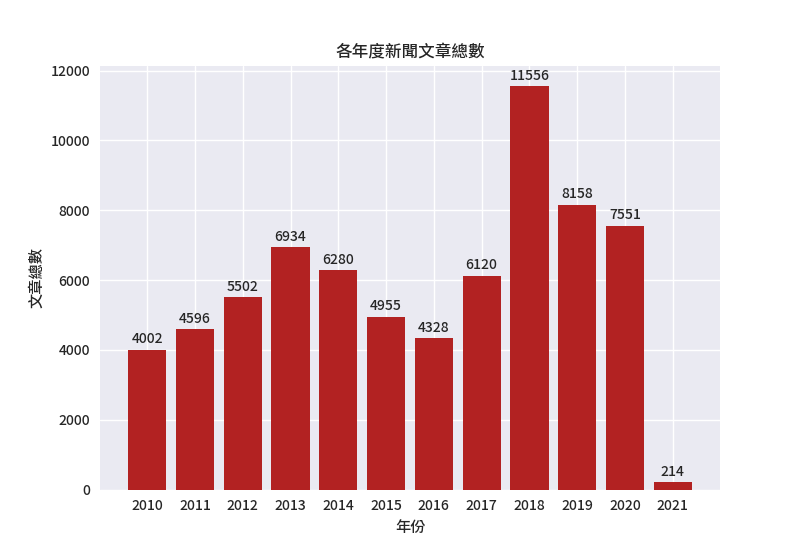
\includegraphics[width=0.7\textwidth]{/Users/chengchanglei/Desktop/CCL/Paper Code/3. Data Description/total_article_num_year.png}
\caption{每年發佈之新聞文章總數時間序列圖}
\end{figure}
圖4.1顯示了2010年1月1號至2021年1月31號之鉅亨網台股新聞資料庫在樣本內所使用之每年新聞文章總數,在樣本中每年平均有6,445篇新聞文章。觀察圖4.1可發現,近年來之新聞數量大於往年之發布新聞數量,顯示近年來非結構化數據之增長。

\begin{figure}[H]
\centering
\includegraphics[width=1.09\textwidth]{/Users/chengchanglei/Desktop/CCL/Paper Code/3. Data Description/output.png}
\caption{新聞文章平均(每日/每半小時)}
\end{figure}
圖4.2上半部繪製了樣本內每天平均發佈之新聞文章數量,由此圖可以看見二月所發布之新聞文章數相較於其他月份來得少,推測可能因為受新年假期以及閏月之影響。下半部則依每半小時為單位,繪製了每半小時平均發佈之新聞數量,從該圖可發現台股開盤時以及開盤後至晚間發布新聞頻率較為頻繁。

\clearpage

\section{資料預處理及統計分析流程}
本節介紹新聞文本資料預處理。中文文本在進行斷詞時,不像英文文本可以透過單詞間的空格直接將新聞文本轉換為單詞儲存即可完成斷詞過程,由於中文文本皆為連續的單詞或詞彙,尚無一套有效之標準流程針對中文文本進行自然語言處理任務的前置作業。

目前中文之自然語言處理以對岸所發明之簡體中文斷詞工具「結巴分詞」 (Jieba) 以及台灣中研院資訊所、語言所成立的語言研究小組針對繁體中文所開發的「中文自然語言處理的資源及研究環境」(Chinese Knowledge and Information Processing, CKIP)。使用者可以利用這些系統對中文文本進行自然語言處理作業,包含斷詞 (Tokenization)、詞性標記 (Part-of-Speech)等自然語言任務。

接著本節將詳細的介紹本研究如何利用自然語言處理之結果對新聞文本進行資料預處理。以下步驟為自然語言處理之正規化(Normalization)流程。第一步將專有名詞移除(如:人名與公司名稱等),由於公司名稱為對應個股股價報酬之標記方式,並假設該篇個股新聞之內容將影響單一個股報酬,因此公司名稱在本次的實驗設計中設定為投資人選擇的個股標籤而非影響股價報酬之詞彙,所以將公司名稱當作專有名詞將其刪除;第二步移除數字、標點符號、特殊符號等非中文詞彙;第三步移除中文停止詞或修飾詞(如:「是」、「的」、「和」等)。最後將所收集到之新聞文章以單詞列表的形式儲存於資料庫中以利後續分析使用。
\subsection{自然語言處理}
本研究在中文斷詞上採用中研院針對『繁體中文』訓練一系列的 Transformer 模型,包含 ALBERT、BERT、GPT2。除了訓練語言模型外, 該系統亦針對各個自然語言任務上訓練了對應的模型(包含斷詞、詞性標記、實體辨識)以資料集中其中一篇文檔做範例如下:
\\[0.6ex]
\begin{tcolorbox}

{\textcolor{blue}{記憶體封測廠力成 (6239-TW) 今(5)日傳出發生氣爆,對此力成回應,僅是3C廠區內發生小事故,但未造成人員傷亡,也沒有對生產或營運造成任何影響。}}
\end{tcolorbox}

\newpage

CKIP斷詞後結果整理如下:
\begin{table}[H]
\begin{center}
\begin{tabular}[c]{l|m{0.3cm}<{\centering}m{0.3cm}<{\centering}m{0.3cm}<{\centering}m{0.5cm}<{\centering}m{0.5cm}<{\centering}m{0.5cm}<{\centering}m{0.3cm}<{\centering}m{0.5cm}<{\centering}m{0.3cm}<{\centering}m{0.3cm}<{\centering}m{0.3cm}<{\centering}m{0.3cm}<{\centering}m{0.5cm}<{\centering}m{0.3cm}<{\centering}m{0.3cm}<{\centering}m{0.5cm}<{\centering}m{0.2cm}<{\centering}m{0.3cm}<{\centering}}
\toprule
單詞& 記憶體 & 封測廠 & 力成 & ( & 6239-TW & ) & 今 & (5) & 日 & 傳出 & 發生 & 氣爆 & , & $\cdots$ & 造成 & 任何 & 影響 & 。 \\
\hline
詞性 & Na & Nb & Nb & Pun. & Neu & Pun. & Nd & Neu & Nd & VC &  VJ & VH & Pun. & $\cdots$ & VK & Vega & Na & Pun. \\
\hline
實體辨識 &  &  & 人物 &  &  & & 日期 & 日期 & 日期 &  &  &  &  &  &  &  &  &  \\
\bottomrule
\end{tabular}
\end{center}
\caption{CKIP斷詞結果}
\label{Tab 4.2}
\end{table}
上述顯示了透過 CKIP 針對繁體中文進行自然語言處理作業之流程,顯示了欲分析之例句以及進行斷詞、詞性標記及實體辨識三種不同之自然語言任務之結果。目的在於辨識出例句中,具有特定意義之單詞,例如,7 月 22 日(日期)、程小明 (人物)、新北市(地點)等具有通俗定義之單詞,而透過實體辨識則可以辨識出目標文本中之專有名詞、時間日期等無情緒詞彙。
\subsection{正規化}
此節詳述了針對繁體中文進行自然語言處理之正規化之過程與結果。正規化 (Normalization) 主要之步驟包含移除『專有名詞』、『日期』等字詞、移除數字、標點符號、特殊符號等非中文詞彙、移除中文停止詞或修飾詞  (e.g., 『和』, 『的』, 『是』, 『也』等),正規化範例如下表格所示:
\begin{table}[H]
\begin{center}
\begin{tabular}[c]{l|m{0.3cm}<{\centering}m{0.3cm}<{\centering}m{0.3cm}<{\centering}m{0.5cm}<{\centering}m{0.5cm}<{\centering}m{0.5cm}<{\centering}m{0.3cm}<{\centering}m{0.5cm}<{\centering}m{0.3cm}<{\centering}m{0.3cm}<{\centering}m{0.3cm}<{\centering}m{0.3cm}<{\centering}m{0.5cm}<{\centering}m{0.3cm}<{\centering}m{0.5cm}<{\centering}m{0.5cm}<{\centering}m{0.2cm}<{\centering}m{0.3cm}<{\centering}m{0.3cm}<{\centering}m{0.3cm}<{\centering}m{0.3cm}<{\centering}}
\toprule
單詞 & 記憶體 & 封測廠 & \textcolor{purple}{力成} & \textcolor{teal}{(} & \textcolor{teal}{6239-TW} & \textcolor{teal}{)} & \textcolor{purple}{今} & \textcolor{purple}{(5)} & \textcolor{purple}{日} & 傳出 & 發生 & 氣爆 & \textcolor{teal}{,} & \textcolor{cyan}{對} & \textcolor{cyan}{此} & \textcolor{purple}{力成} & 回應 \\
\hline
詞性 & Na & Nc & Nb & Pun. & Neu & Pun. & Nd & Neu & Nd & VC &  VJ & VH & Pun. & P & Nep & Nb & VC \\
\hline
實體辨識 &  &  & 人物 &  &  & & 日期 & 日期 & 日期 &  &  &  &  & \\
\bottomrule
\end{tabular}
\end{center}
\caption{CKIP正規化結果}
\label{Tab 4.3}
\end{table}

\begin{table}[H]
\begin{center}
\begin{tabular}[c]{l|m{0.5cm}<{\centering}m{0.3cm}<{\centering}m{0.5cm}<{\centering}m{0.5cm}<{\centering}m{0.3cm}<{\centering}m{0.5cm}<{\centering}m{0.3cm}<{\centering}m{0.5cm}<{\centering}m{0.5cm}<{\centering}m{0.5cm}<{\centering}m{0.3cm}<{\centering}m{0.3cm}<{\centering}m{0.5cm}<{\centering}m{0.3cm}<{\centering}m{0.5cm}<{\centering}m{0.5cm}<{\centering}m{0.2cm}<{\centering}m{0.3cm}<{\centering}m{0.3cm}<{\centering}m{0.3cm}<{\centering}m{0.3cm}<{\centering}}
\toprule
單詞 & \textcolor{teal}{,} & \textcolor{cyan}{僅} & \textcolor{cyan}{是} & \textcolor{teal}{3C} & 廠區 & \textcolor{cyan}{內} & 發生 & \textcolor{cyan}{小} & 事故 & \textcolor{cyan}{但} & \textcolor{cyan}{未} & 造成 & 人員 & 傷亡 & \textcolor{teal}{,} & \textcolor{cyan}{也} & 沒有 \\
\hline
詞性 & Pun. & Da & SHI & FW & Nc & P & VC & VH & Na & Cbb & D & VK & Na & VH & Pun. & D & D \\
\hline
實體辨識 &  &  &  &  &  & &  &  &  &  &  &  &  & \\
\bottomrule
\end{tabular}
\end{center}
\caption{CKIP正規化結果}
\label{Tab 4.4}
\end{table}

\begin{table}[H]
\begin{center}
\begin{tabular}[c]{l|m{0.5cm}<{\centering}m{0.5cm}<{\centering}m{0.5cm}<{\centering}m{0.5cm}<{\centering}m{0.5cm}<{\centering}m{0.7cm}<{\centering}m{0.5cm}<{\centering}m{0.5cm}<{\centering}}
\toprule
單詞 & \textcolor{cyan}{對} & 生產 & \textcolor{cyan}{或} & 營運 & 造成 & 任何 & 影響 & \textcolor{teal}{。} \\
\hline
詞性 & P & VC & Caa & VA & VK & Neqa & Na & Pun. \\
 \\
\hline
實體辨識 &  &  &  &  &  &  &  & \\
\bottomrule
\end{tabular}
\end{center}
\caption{CKIP正規化結果}
\label{Tab 4.5}
\end{table}

第一步移除專有名詞(上表標註之紅色單詞),此步驟根據實體辨識結果,移除 CKIP 可辨識之特定意義詞彙(e.g., 組織:力成; 人名:張忠謀; 日期: 5 日、上午 9 時; 地名: 台北市、臺灣, etc.),透過該系統可移除文本中大量專有名詞,解決了中文自然語言處理一大難處。

第二步為移除數字、標點符號及特殊符號等非中文詞彙(上表標註為綠色之單詞),此步驟利用詞性標記及特殊符號字典交互進行,移除詞性被標記為「數 字」、「標點符號」、「英文」亦或該單詞存於特殊符號字典中之詞彙。

第三步為移除中文停止詞或修飾詞(上表標註為藍色之單詞),中文停止詞與修飾詞(e.g.「和」、 「的」、「是」、「也」etc.)在中文上無特殊意義,保留此類單詞易造成模 型有過多噪音。至此,可完成正規化作業。

\newpage

\subsection{資料預處理與統計分析流程}

\begin{figure}[htbp]
\centering
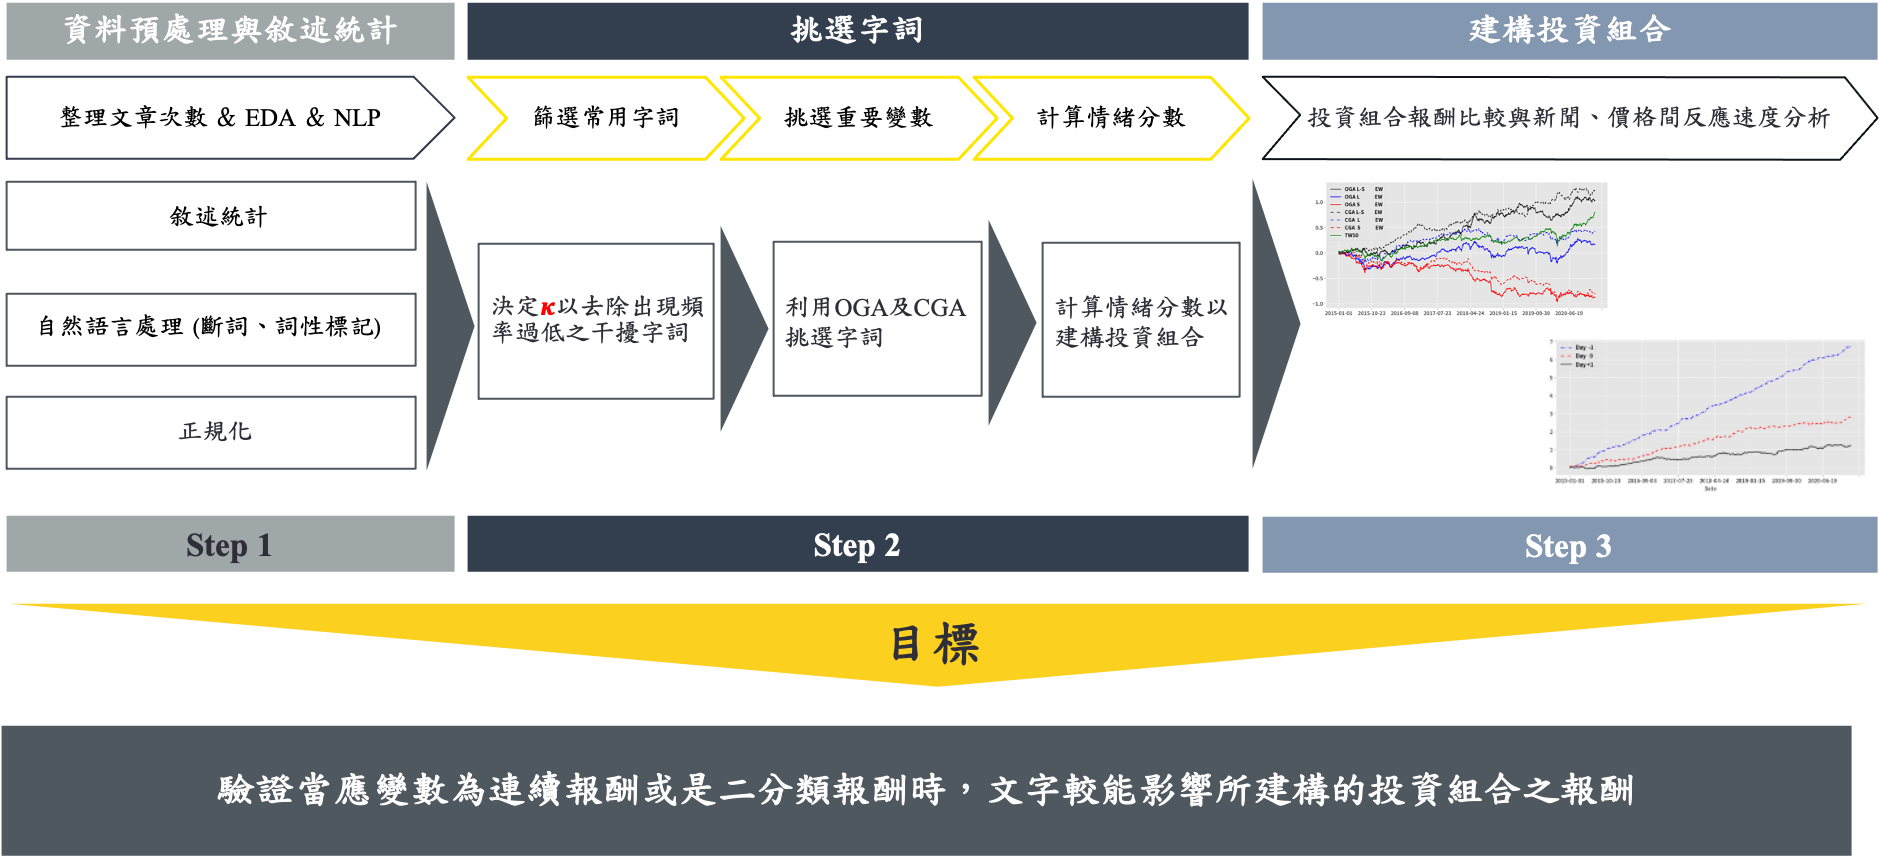
\includegraphics[width=1.1\textwidth]{images/流程圖.png}
\caption{統計分析流程圖}
\end{figure}



\section{實證結果}
本節將建構台股新聞情緒模型,以計算每日情緒分數並建構交易策略及投資組合,進而實證當應變數報酬為線性假設或者是非線性假設時,何者能有較好的超額報酬。以及驗證在散戶為主的台灣市場中之間隔延遲關係,並透過在不同條件之下(市值、波動度)探討台灣股市之新聞反應速度。
\subsection{預測股票報酬}
此小節將詳述如何訓練模型並估算每日新聞情緒分數。以五年為一個滾動(rolling)週期,樣本內前五年用於訓練,同時根據滾動週期,使用樣本週期後一年進行樣本外測試(ex:第一個rolling為2010年至2014年,並利用2015年進行測試)。在每次測試年份結束後,將整個訓練週期向後滾動一年並重新訓練模型,直到用盡所有樣本資料為止。完成模型訓練及情緒分數估算後,透過估算出之情緒分數建構隔日投資組合,參考 Ke, Kelly, and Xiu (2019) 將台灣時間 09:00 a.m. 至隔日 09:00 a.m. 時間區間定義為一天,並且將 Day 0所蒐集之新聞文章計算情緒分數後,用以建構隔日投資組合。當中將台灣時間 08:30 a.m. 至 09:00 a.m.所發佈之新聞移除不用於測試集交易,其目的在於希望模型用於測試集交易時能更加的貼近真實情況,例如基金公司於開盤前便已針對前一天所發佈之新聞決定當日部位變動,若使用過於接近開盤時所發佈之新聞,可能造成基金公司或投資人沒有充足的時間計算部位以因應在流動性高峰期間進行交易。

本研究針對Day 0所發佈之個股新聞,將於Day 1開盤時建構投資組合部位,並於隔日開盤時將所持有的部位平倉,稱為隔日報酬投資組合。由上述做法,每天開盤都會建構新的投資組合,並持有部位1天,使用此種策略原因主要有以下兩點:第一,於收盤過夜期間所發佈之新聞,最可能於隔日市場開放的早期影響股票價格,因為該段時間是大多數交易者進入市場的時間。第二,除了從事高頻交易基金的公司之外,其餘基金公司之風險控管及資金限制等因素,不太可能根據盤中才出現的新聞消息而不斷地調整部位,因此透過衡量新聞對於隔日報酬的影響,能有效地得知前一天所發佈之新聞是否能影響投資人決策而影響股價。

\begin{figure}[htbp]
\centering
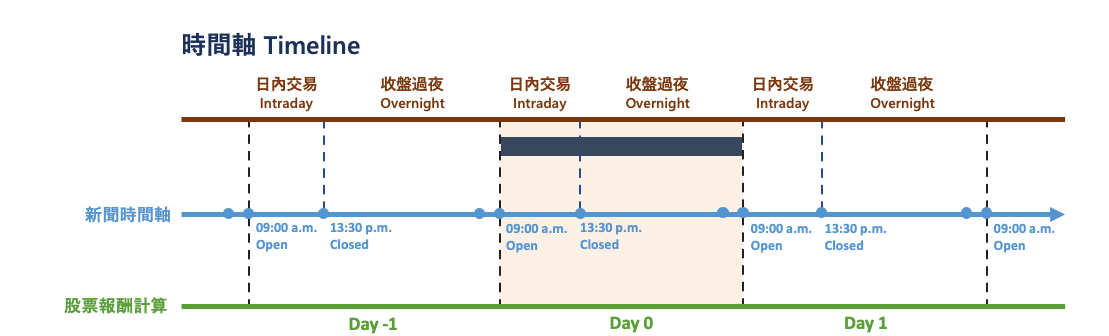
\includegraphics[width=1.1\textwidth]{images/times.png}
\caption{交易時間軸}
\end{figure}


\subsection{字詞挑選結果}
\begin{figure}[htbp]
\centering

\includegraphics[width=1.1\textwidth]{images/OGA result.png}
\caption{OGA 字詞挑選結果}
\end{figure}

\begin{figure}[htbp]
\centering

\includegraphics[width=1.1\textwidth]{images/CGA result.png}
\caption{CGA 字詞挑選結果}
\end{figure}
圖4.5與圖4.6分別為OGA以及CGA所挑選出來與報酬最相關之正面與負面情感詞,由於訓練週期會不斷改變,且會重新估算情緒分數,因此分析過程中,情感詞列表也會不斷地改變。如前述所說本研究共有兩種參數$\kappa$ 與 $k$,而本研究參考Fan, et al.(2021)之實證流程,由70\%至90\%且每2\%為一間隔挑選$\kappa$;而$k$則由100至500進行實證分析。我們找出報酬最高之參數為代表進行後續之實證分析。上述兩圖以投資組合中報酬最高為代表所挑出之情感詞。


\subsection{投資組合報酬比較}
本研究藉由情緒分數模型建構一日交易策略,我們蒐集第T天所發佈之新聞文章,並估算第T天所有新聞文章之情緒分數,並將所估算之情緒分數於第T+1天開盤時建構投資組合。於投資組合的多頭部位買進情緒分數最高的5篇新聞所對應之五檔公司股票,於投資組合的空頭部位則賣出情緒分數最低的5篇新聞所對應之五檔公司股票。除此之外,也考慮等權重(Equal-Weight, EW)及市值權重(Value-Weight, VW)兩種不同買賣方式之投資組合績效,等權重將所持有資金「等比例」配置於所持有之五檔作多股票及五檔作空股票;市值權重則將所持有資金依「市值」配置於所持有之五檔作多股票及五檔作空股票。在評估績效方面,我們考慮了等權重多空部位(EW L-S)、等權重多頭部位 (EW L)、等權重空頭部位(EW S)、市值權重多空部位(VW L-S)、市值權重多頭部 位(VW L)、市值權重空頭部位(VW S),總共六種不同的配對投資組合策略,將相同策略進行比較(多空策略與多空策略比較、多頭策略與多頭策略比較、空頭策略與空頭策略比較),並將以上投資組合與買進並持有(Buy and Hold)臺灣50相比較,最後透過評估投資組合績效確認基於情緒分數模型所建構之投資組合策略是否有顯著超額報酬。

\newpage

\begin{figure}[htbp]
\centering
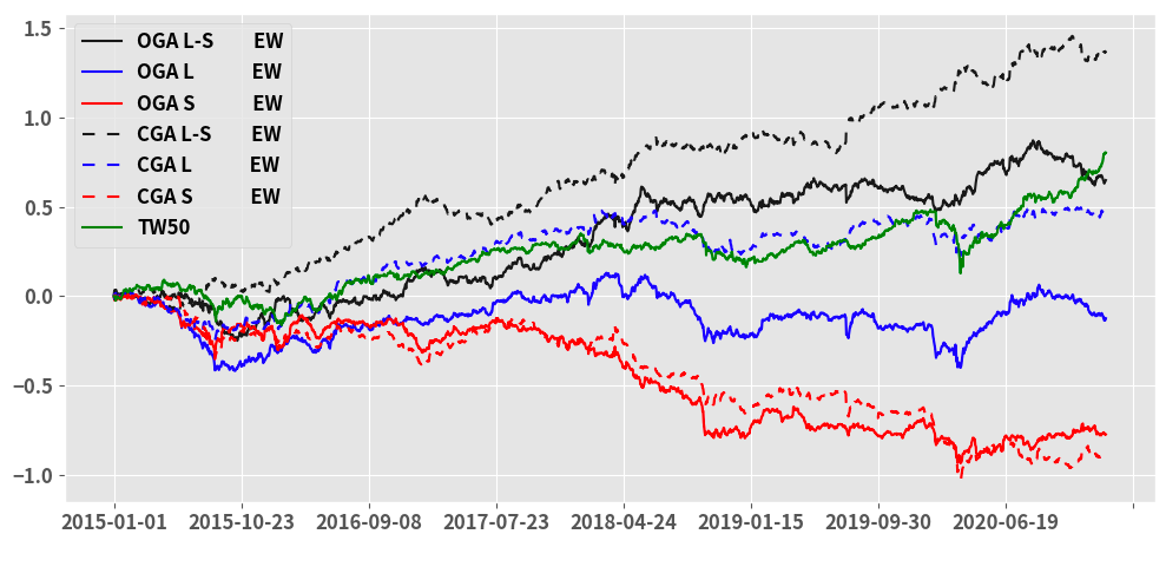
\includegraphics[width=1.1\textwidth]{images/OGA vs CGA.png}
\caption{OGA v.s CGA}
\end{figure}

於圖4.7繪製了利用情緒分數所建構之投資組合其「樣本外」累積對數報酬。黑線、藍線及紅線分別表示多空部位(Long-Short)、多頭部位(Long)及空頭部位(Short)之投資組合。實線及虛線則分別表示OGA及CGA兩種不同之模型假設之投資組合績效。綠色實線表示買進並持有臺灣50 (TW50)之報酬。而以夏普值(Sharpe Ratio)以及平均報酬(Average Return)來看,不管在多空策略、多頭策略或者是空頭策略上,CGA Predict皆比OGA Predict來得好,所以在接下來的分析之中皆以CGA所建構之情緒分數模型進行以下的實證分析。
\begin{table}[H]
\begin{center}
\begin{tabular}[c]{m{5cm}<{\centering}m{5cm}<{\centering}m{5cm}<{\centering}}
\toprule
 & 夏普值  & 平均報酬 \\
交易策略 & Sharpe Ratio & Average Return \\
\hline
OGA EW L-S & 0.52 & 3.33 \\
OGA EW L & -0.11 & -0.64 \\
OGA EW S & 0.73 & 3.97 \\
CGA EW L-S & 1.18 & 6.97 \\
CGA EW L & 0.45 & 2.36 \\
CGA EW S & 0.83 & 4.61 \\
TW 50    & 0.74 & 4.12 \\
\bottomrule
\end{tabular}
\end{center}
\caption{新聞情緒分數投資組合表現}
\label{Tab 4.6}
\end{table}

\newpage

\begin{figure}[htbp]
\centering
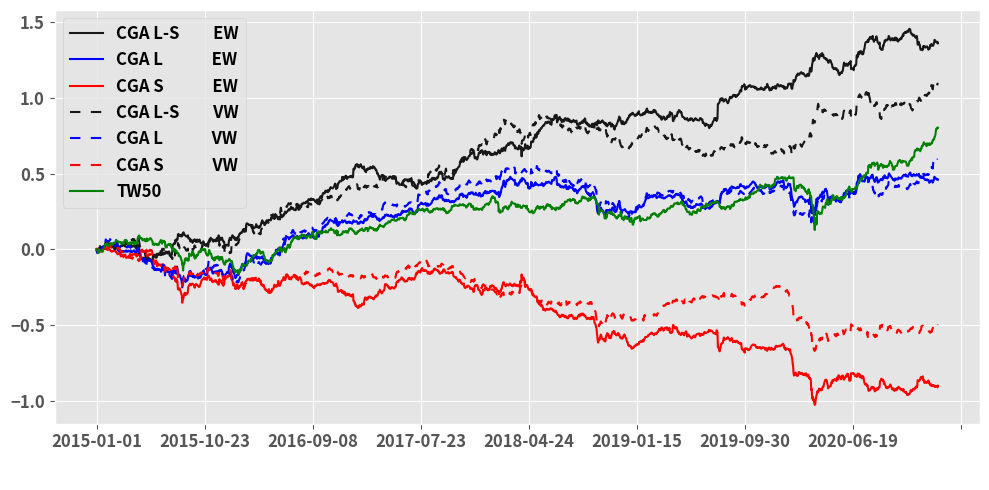
\includegraphics[width=1.1\textwidth]{images/CGA all.png}
\caption{CGA投組積效}
\end{figure}
於圖4.8繪製了利用CGA Predict所建構之投資組合「樣本外」累積對數報酬。黑線、藍線及紅線分別表示多空部位(Long-Short)、多頭部位(Long)及空頭部位(Short)之投資組合。實線及虛線則分別表示等權重(Equal-Weighted)及市值權重(Value-Weighted)兩種不同交易方式之投資組合績效。綠色實線表示買進並持有臺灣 50 (TW50)之報酬。根據上圖我們有以下三點結論,第一,我們可以看到在等權重以及市值權重中空頭部位之績效皆優於多頭部位之績效,我們做出以下之解釋:因為本研究只要研究台灣股市之市場,而台灣股市是一個以散戶為主之市場,而散戶交易人對於負面新聞較為敏感,若出現不利於所持有股票之新聞,較傾向受情緒左右而賣出部位,也顯示了散戶不理性之心態。第二,等權重投組之績效優於市值權重投組之績效,此結果顯示了在不考慮其他條件時,透過新聞文章所量化之情緒分數能較好的預測小型股票之報酬,我們針對此結果有以下解釋(1)投資者對於小型股票關注度較低且流動性不足等因素,因此新聞反應速度較慢。(2)小型股票之基本面相較於大公司之不確定性較為強烈,因此需要更多時間分析其新聞資訊。(3)大型股票受較多人研究與關注,所以其股價較不受新聞情緒因子所影響。第三,使用CGA Predict所建構之交易策略,於等權重多空部位投資組合以及市值權重多空部位投資組合,皆優於買進並持有臺灣50。

我們也檢驗了本研究所建構出新聞情緒因子是否會被Fama, French(1993)所提出之三因子以及Fama, French(2015)所提出之五因子解釋,根據表4.7可以發現,在所有三因子與五因子檢驗中之$R^{2}$皆小於$\alpha = 0.05$,亦即解釋能力皆為不顯著。
\begin{table}[H]
\begin{center}
\begin{tabular}[c]{cccm{1cm}<{\centering}m{1cm}<{\centering}m{1cm}<{\centering}m{1cm}<{\centering}m{1cm}<{\centering}m{1cm}<{\centering}}
\toprule
交易策略 & 夏普值  & 平均報酬 & FF3 &  & FF5 &  & FF5 + MOM & \\

Strategy & Sharpe Ratio & Average Return & $\alpha$ &  $R^{2}$  & $\alpha$ &  $R^{2}$ & $\alpha$ &  $R^{2}$ \\
\hline
CGA EW L-S & 1.18 & 6.97 & 7 & 0.6 & 7 & 0.7 & 7 & 0.7 \\
CGA EW L & 0.45 & 2.36 & 1 & 0.2 & 1 & 0.2 & 1 & 0.3\\
CGA EW S & 0.83 & 4.61 & 6 & 0.7 & 6 & 0.8 & 6 & 0.8\\
CGA VW L-S & 0.92 & 5.59 & 5 & 0.2 & 4 & 0.2 & 5 & 0.2\\
CGA VW L & 0.55 & 3.05 & 1 & 0.2 & 1 & 0.3 & 0.95 & 0.3\\
CGA VW S & 0.49 & 2.54 & 3 & 0.3 & 3 & 0.3 & 4 & 0.3\\
\bottomrule
\end{tabular}
\end{center}
\caption{三因子/五因子檢驗結果與CGA投資組合表現}
\label{Tab 4.7}
\end{table}
\footnotetext[1]{$R^{2}$單位:\%}
\subsection{新聞與價格延遲之關係與反應速度}
參考 Ke, Kelly, and Xiu (2019) 與 Fan, Xue, and Zhou (2021)近一步比較股票價格與新聞發佈時間之領先滯後關係。於訓練樣本中使用第T天所發佈之新聞對應至第T天之股票報酬訓練模型後分析樣本外第T天之新聞情緒與 T-1 天股票報酬 (第 T-1 天開盤至第 T 天開盤)、第 T 天股票報酬以及第 T+1 天股票報酬之間的關係,以 Day +1 ,Day -1 及 Day 0 三種不同的策略進一步的分析,探討台股市場中,投資人對於新聞消息之反應是否具有差異性,以及投資人是否有可能在新聞正式發佈以前便已經掌握未發布之新聞消息。
\begin{figure}[htbp]
\centering
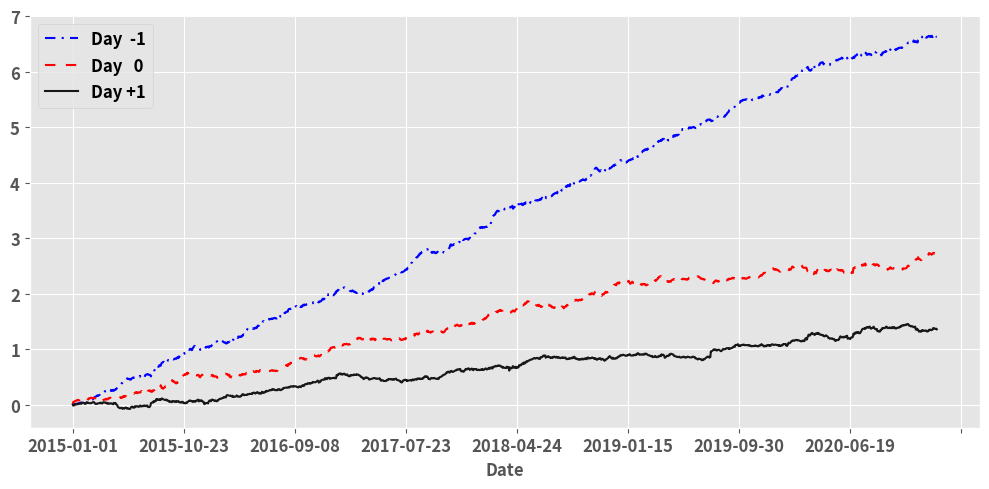
\includegraphics[width=1.1\textwidth]{images/speed0.png}
\caption{新聞情緒與價格延遲之關係}
\end{figure}

\newpage

在本小節我們比較了股票價格與新文發佈時間的關係,圖4.9分析了「樣本外」第 T 天新聞情緒與 T-1 天股票報酬、第 T 天股票報酬及第 T+1 天股票報酬之間的關係。Day -1 (藍色虛線) 為新聞情緒與新聞發佈前一天股票報酬之間的關係,而臺股於Day-1反應劇烈,顯示有部分報酬已透過內線反應至股價當中,意即市場上某些投資在新聞發布前便已知曉信息。Day 0 (紅色虛線)則為新聞情緒與發佈當天股票報酬之間的關係,可以發現大部分新聞訊息皆於新聞發布前後反應至股價當中,但是以上兩種策略為無法執行之交易策略,其所獲得之報酬為新聞發佈前之投資報酬,投資人於實盤交易之中無法於此二時段進行交易。

Day +1 (黑色實線)為新聞情緒與發佈隔天股票報酬之間之關係,為可行之交易策略,顯示了新聞情緒的延遲程度,該策略量化新聞情緒反應至股價中之「延遲程度」,可以看到 Day +1 策略仍可以帶來超額報酬,此結果顯示利用情緒因子所建構之投資組合仍然可以帶來超額報酬。


\subsection{異質性分析}
驗證領先滯後關係後本研究欲更深入針對不同類型股票之新聞反應時間進行異質性分析 (Heterogeneity Analysis),目的在於了解不同類型新聞之價格反應情形,欲使用市值與波動度兩個變數。使用市值之原因在於,因市值較大的公司代表著投資人將較多的資產分配於該公司股票,並且投資者容易將更多的注意力專注於大公司新聞 (Wilson (1975)、Veldkamp (2006))。因此基於每個時期台股上市公司市值中位數將股票分為大公司及小公司,並根據大小公司繪製每日平均報酬進行情緒訊息反應之比較分析,驗證投資者注意力之多寡是否影響相關新聞消息之反應。

再者使用波動度之原因在於,波動度係為套利交易之極限,在其他條件皆相同的情況下,股票波動度越高代表股票報酬的不確定性就越大。隨著更多的不確定性下,及可能使擁有越豐富資訊之投資者能獲得更高的報酬。然而,更多的不確定性也可能使該新聞之訊息較較難以被解釋,新聞所包含的情緒反應至股價之速度也較為緩慢。為驗證此現象也預計基於每個時期台股上市公司波動度中位數將股票分為高波動公司及低波動公司,並同樣根據高低波動公司繪製每日平均報酬進行比較分析。

\newpage

\begin{figure}[htbp]
\centering
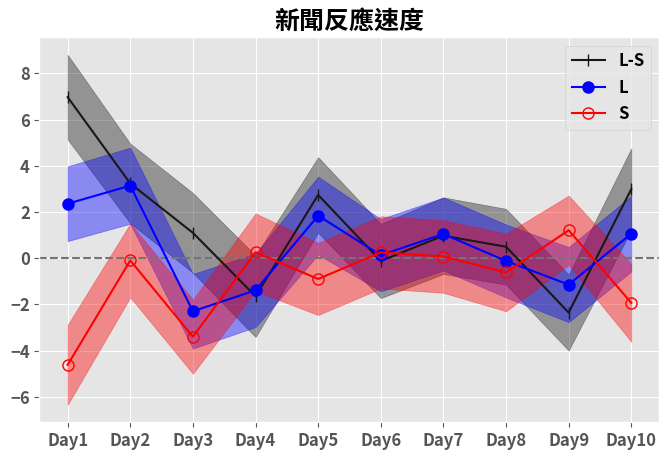
\includegraphics[width=1.1\textwidth]{images/speed1.png}
\caption{新聞反應速度}
\end{figure}

圖4.10繪製了用新聞情緒分數所建構之投資策略在新聞發佈後 1 至 10 日持有一日之每日平均報酬。如 Day 4 表示於新聞發佈後四日進行情緒分數交易策略之平均報酬(Average Returns)。陰影部分則為每日平均報酬之 95\%信賴區間。

本小節將進一步分析在延遲閱讀新聞下,進行情緒分數交易策略,則新聞情緒延遲反應之情形。圖4.10中繪製多空部位投資組合(Long-Short)以及多頭部位(Long)及空頭部位(Short)投資組合,圖中可發現對於多空策略,新聞情緒訊息於 Day+3時已經完全反應至股價當中。與美股市場不同的是,根據 Ke, et al. (2019) 研究顯示,美股新聞情緒訊息可以延續至Day+4始能反應完畢,顯示臺灣新聞情緒訊息大多於新聞發佈日或發佈前一天便提早反應至股價當中。

\newpage

\begin{figure}[htbp]
\centering
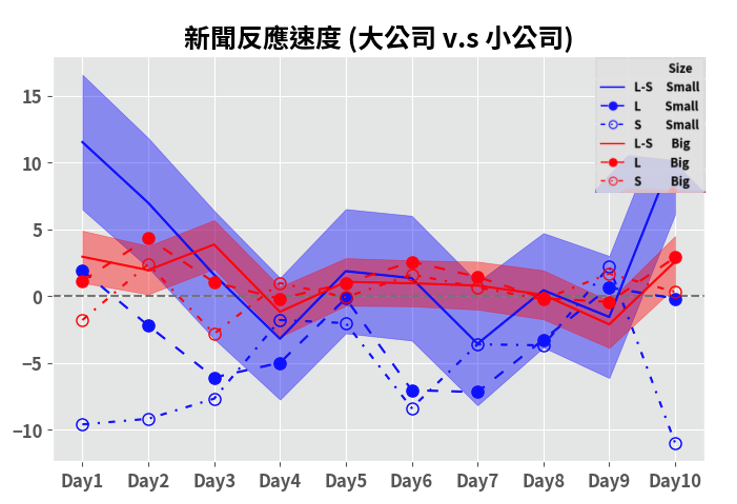
\includegraphics[width=1.1\textwidth]{images/speed2.png}
\caption{新聞反應速度(大公司 v.s 小公司)}
\end{figure}
圖4.11根據公司市值區分大公司及小公司繪製每日平均報酬(Average Returns)。區別大小公司之依據為利用每個時期台股上市公司市值中位數進行劃分。圖4.11中可發現小公司多頭部位在Day +1皆反應完畢,顯示了即便小公司出現正面新聞,投資者仍然較不傾向購入小公司之股票。小公司空頭反應至Day +4,顯示一旦小公司出現負面新聞,投資者傾向積極賣出小公司之股票,顯示了投資者之恐慌心理。大公司空頭於Day +1即反應完畢,顯示負面新聞較不影響投資人對於大公司股票持有之態度。

\newpage

\begin{figure}[htbp]
\centering
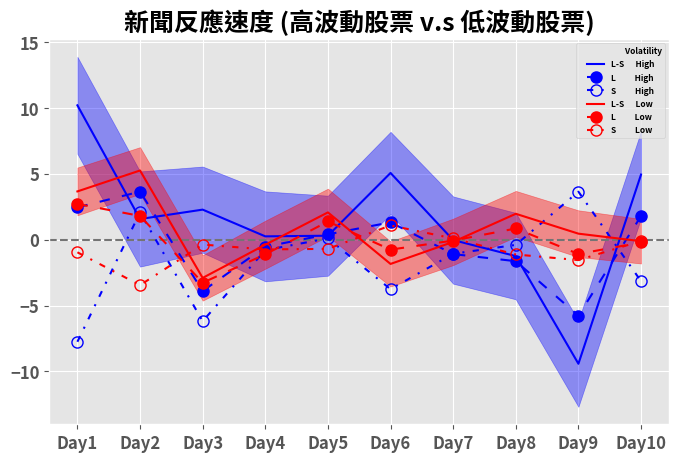
\includegraphics[width=1.1\textwidth]{images/speed3.png}
\caption{新聞反應速度(高波動 v.s 低波動)}
\end{figure}
圖4.12根據股票波動度區分高波動及低波動股票繪製每日平均報酬(Average Returns)。區別高低波動度股票之依據為每時期台股上市公司股票波動度中位數進行劃分。圖4.12可以發現,波動度越高,股票報酬之不確定性就越大,而隨著更多不確定性的產生,擁有更多資訊之投資者即可能獲得較高之報酬。然而,更多的不確定性代表該新聞訊息較難以被解釋,因此,新聞所包含的情緒訊息反應至股價的速度也較為緩慢,可以看到高波動公司需要三天才能將情緒完全反應至股價中。














\chapter{結論與建議}
\label{c:experiment}

\section{結論與建議}
本研究主要依據 Ing and Lai (2011) 及 Chen, Dai, Ing, Lai (2019)所改良之高維度選模模型之文字探勘方法建構台股新聞情緒分數模型,本研究利用模型估算新聞情緒分數而建構交易策略,並評估當應變數為線性假設及非線性假設下投資組合報酬之優劣及新聞反應速度之差異,以驗證散戶為主之台股市場之投組表現。

進行實證分析後發現,透過兩種不同的高維度選模模型所估算的新聞情緒分數確實能有效地預測台股報酬,且當應變數為非線性假設之報酬時能得到更好的投資組合報酬。該情緒分數能精確地捕捉新聞情緒,也能幫助投資者更好的理解新聞媒體是如何影響投資人的交易決策的。在實證分析中我們透過新聞與價格之延遲關係發現,與美國相比,臺灣股票市場在新聞訊息傳遞的速度上有明顯差異,此結果也符合Ke et al. (2019)所提出之結論。除此之外,透過新聞反應速度的分析發現,臺灣的投資人(散戶為主的市場)結構與美國(法人為主的市場)確實有很大差異,此差異為在進行投資決策時,臺灣投資人多有過度悲觀與恐慌反應的情形發生,導致與看見正面新聞而買進股票相比,臺灣投資人更傾向於當負面新聞出現時將股票賣出,此現象也反應在投資組合的報酬之中,也就是與多頭策略相比,空頭策略能夠得到較好的報酬。

本研究最主要目的為驗證當應變數報酬為線性假設或者是非線性假設時,何者可以得到更好的超額報酬並驗證台灣股票市場中之散戶於市場中之反應與績效表現。根據實證結果發現,利用本研究之模型所估算之情緒分數作為投資組合建構依據,其績效優於大盤,也顯示了新聞媒體對於臺灣股票市場不具效率性。對於未來研究方向,除了希望能使用更長期的新聞資料進行研究分析外,也希望能夠解決當新聞文章標註多家公司的問題。
\chapter{參考文獻}
\begin{itemize}
\item 郭亭佑. (2021). 透過文字探勘預測台股報酬. \textit{政治大學金融學系學位論文}
\item Blei, D. M., Ng, A. Y., and Jordan, M. I. (2003). Latent dirichlet allocation. \textit{Journal of Machine Learning Research, 3,}993-1022
\item Chen, Y. L, Dai, C. S and Ing, C. K (2019). High-dimensional model selection via Chebyshev greedy algorithms. Working paper.
\item Fan, J., Xue, L., and Zhou, Y. (2021). How much can machines learn finance from Chinese text data?. Working Paper.
\item Gentzkow, M., Kelly, B., and Taddy, M. (2019). Text as data. \textit{Journal of Economic Literature, 57 }(3), 535-74.
\item Henry, E. (2008). Are investors influenced by how earnings press releases are written?. \textit{The Journal of Business Communication, 45}(4), 363–407.
\item Ing, C. K., and Lai, T. L. (2011). A stepwise regression method and consistent model selection for high-dimensional sparse linear models. \textit{Statistica Sinica}, 1473-1513.
\item Jegadeesh, N., and Wu, D. (2013). Word power: A new approach for content analysis. \textit{Journal of Financial Economics, 110(3)}, 712-729.
\item Ke, Z. T., Kelly, B. T., and Xiu, D. (2019). Predicting returns with text data. Working Paper.
\item Loughran, T., and McDonald, B. (2011). When is a liability not a liability? Textual analysis,
dictionaries, and 10-Ks. \textit{Journal of Finance, 66}(1), 35-65.
\item Manela, A., and Moreira, A. (2017). News implied volatility and disaster concerns. \textit{Journal of Fi-
nancial Economics, 123(1)}, 137–162.
\item Temlyakov, V. N. (2015). Greedy approximation in convex optimization. \textit{Constructive Approxima- tion, 41}(2), 269-296.
\item Tetlock, P. C. (2007). Giving content to investor sentiment: The role of media in the stock market. \textit{The Journal of Finance, 62}(3), 1139-1168.
\item Tibshirani, R. (1996). Regression shrinkage and selection via the lasso. \textit{Journal of the Royal Statistical Society: Series B (Methodological), 58}(1), 267-288.
\item You, J., Zhang, B., and Zhang, L. (2018). Who captures the power of the pen?. \textit{Review of Financial Studies, 31}(1), 43–96.
\end{itemize}


































\@startappendix

% \input{chapters/dataset}

\backmatter

\clearpages
\phantomsection
\addcontentsline{toc}{chapter}{\bibname}
\bibliographystyle{apa}

% Your bibliography goes here
\bibliography{thesis.bib}

\end{document}
